\section{Proposed Method}
\label{sec:propwork-casod-method}

%\sysb resembles \sysa in that a MVCNN is used for the FgBg multi-view model $f_{MV}$ backbone. Each feature extractor $\phi_v = f_{\theta,v}$ (parameterized by $\theta$) outputs a $d$-dimensional feature vector from input view $x_v$, $\phi_v: \mathcal{X} \mapsto \mathbb{R}^d$. The multi-view feature extractors $\phi_{MV}$ give $Z_{MV} = \{z_{org}, z_{fg}, z_{bg}\}$ with corresponding classification parameters $W_{MV}$ and $b_{MV}$ subsequently outputting $\hat{Y}_{MV} = \{\hat{y}_{org}, \hat{y}_{fg}, \hat{y}_{bg}\}$. The fusion component $\mathcal{U}$ in \sysb differs significantly from \sysa, instead constructing the single-view features, cross-view features, and comprehensive fused feature for ensembling.
\gls{sys} deviates from the architectures of \gls{sysa} and \gls{sysb}. The FgBg multi-view model $f_{MV}$ is now composed of a single pre-trained Vision Transformer (VIT) \cite{dosovitskiy2020image} feature extractor with three sets of Adapter \cite{hu2021lora} modules. Each Adapter set is \textit{view-specific}, that is each view exclusively passes through its own Adapter set. These Adapter modules (or Adapters), along with the shared VIT, are delineated as feature extractor $\phi_v = f_{\theta,v}$ for view $v$. As before, the multi-view feature extractors $\phi_{MV} = \{\phi_{org}, \phi_{fg}, \phi_{bg}\}$ and corresponding classification layers $W_{MV}$, $b_{MV}$ give view-specific feature $Z_{MV}$ and prediction logits $\hat{Y}_{MV}$. The \gls{sys} fusion component $\mathcal{U}$ introduces a unique attention-based fusion methodology based on \gls{cvca} and hierarchical combination of correlated, view-informed features.


\begin{figure*}
	\centering
	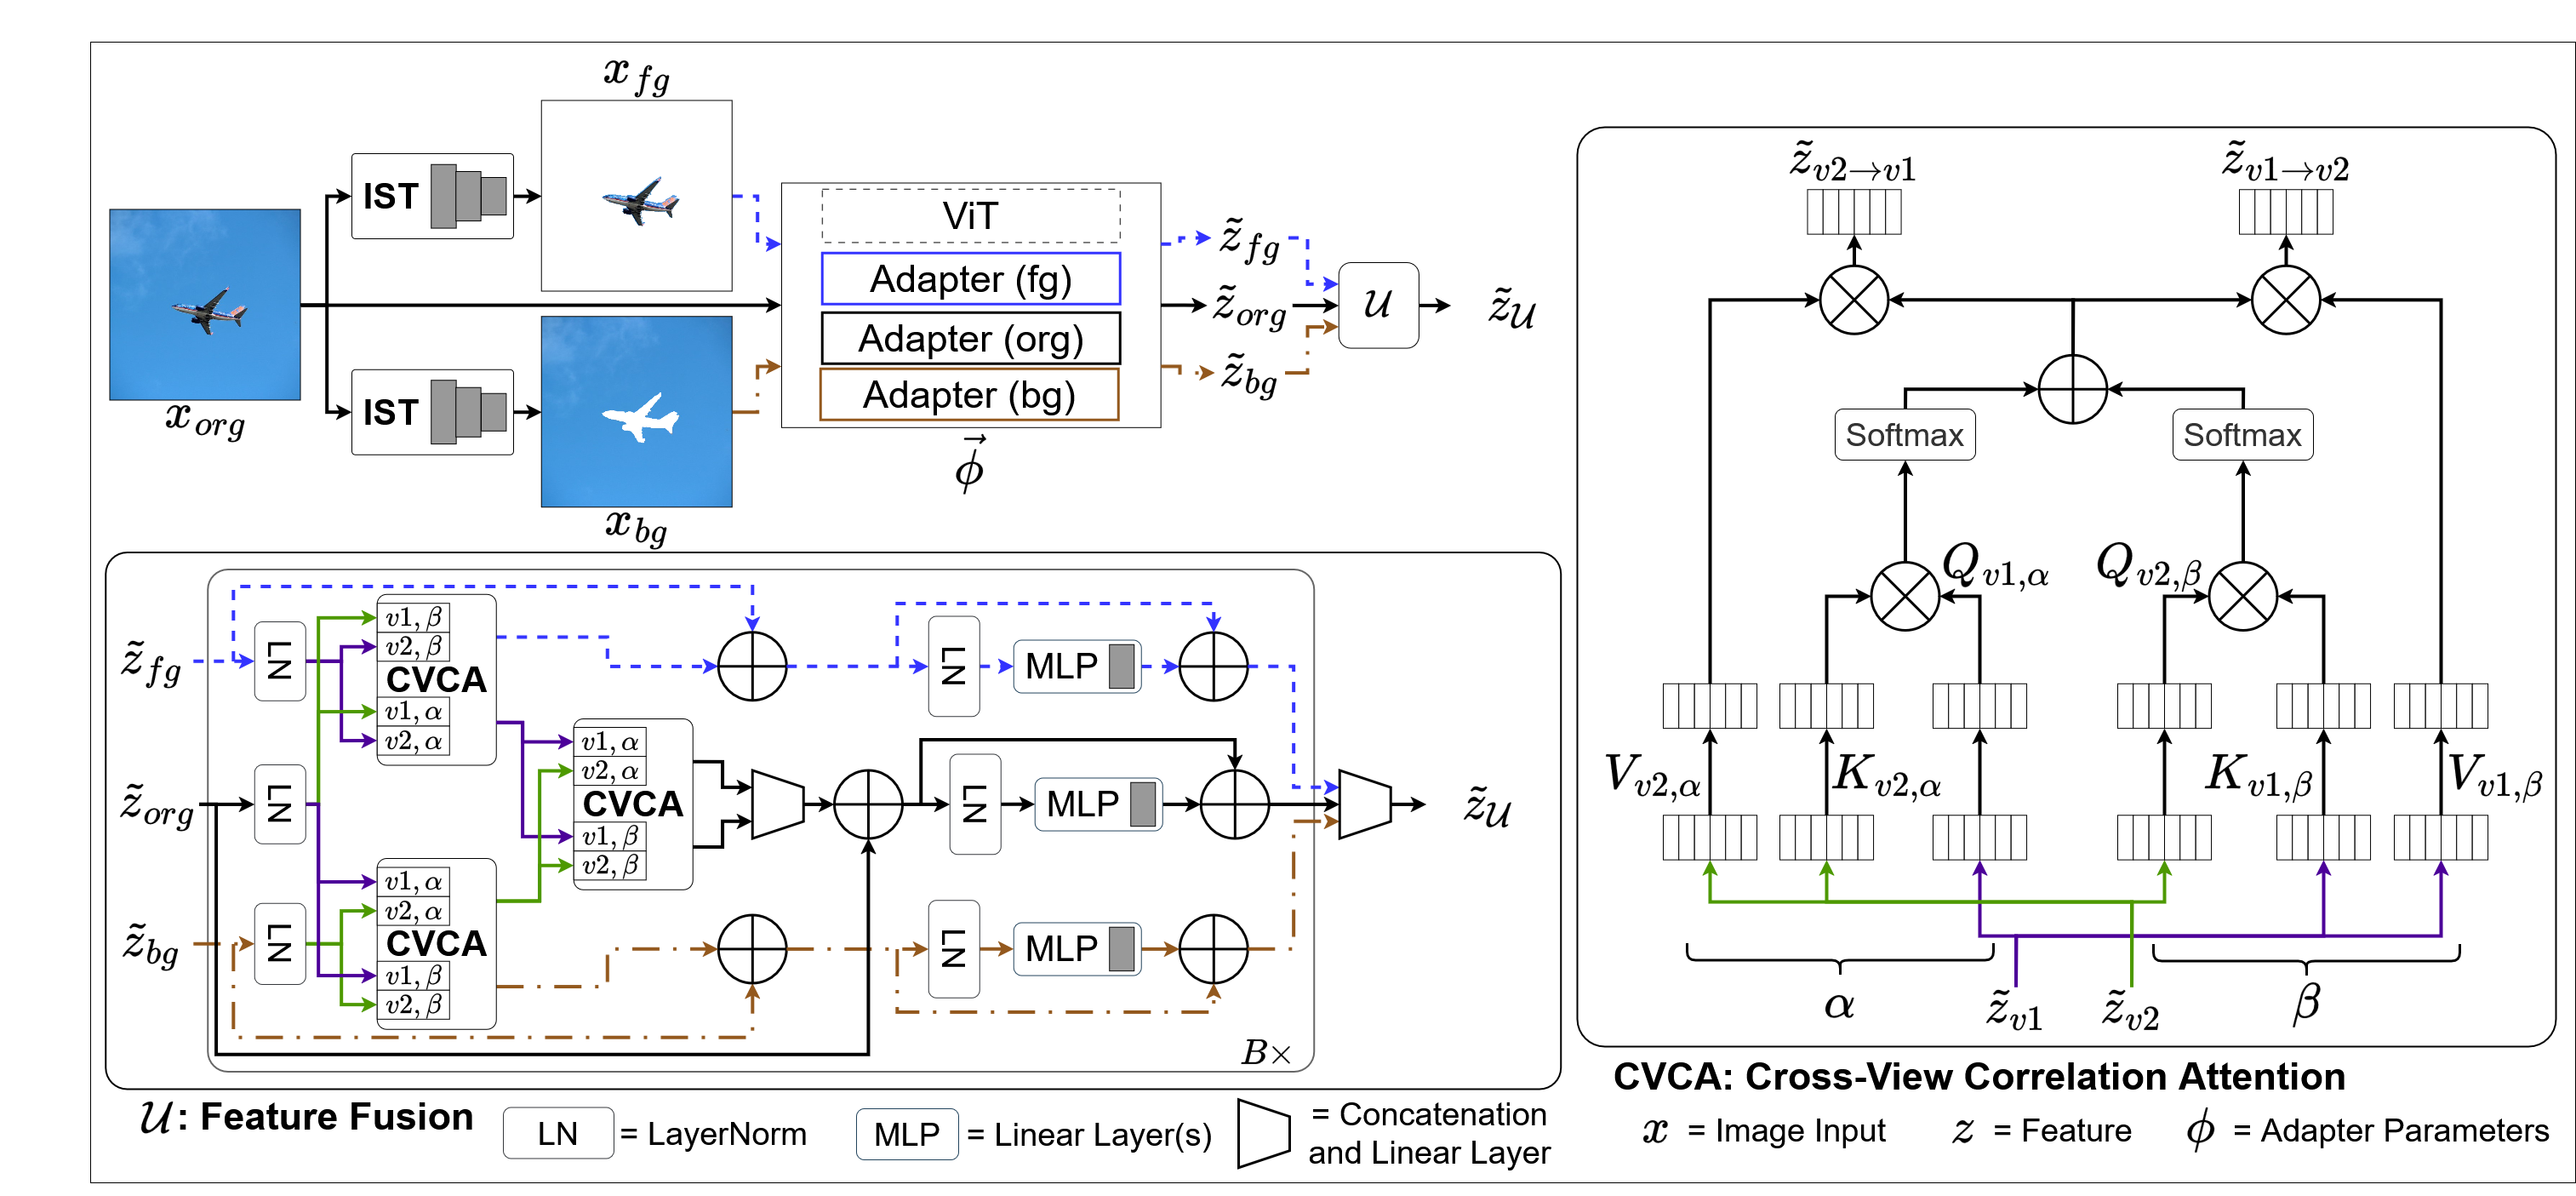
\includegraphics[width=1.\linewidth]{figures/casod_diagram}
	
	\caption{Model architecture of the proposed \sys. 
		%Black lines refer to the original or fused image features. Blue lines refer to foreground image features, orange lines refer to background image features. Best viewed in color. 
        $\alpha$ and $\beta$ are illustrative cues that connect views to CVCA modules.
	}
	\label{fig:casod_model_arch}
\end{figure*}

%Let $\mathcal{D}_{id} = \{(x_i, y_i)\}_{i=1}^N$ be the ID image classification dataset, where $y_i$ is the class label of image $x_i$, and $\mathcal{Y} = \{y_1, y_2, ... , y_R\}$ be the set of all ID class labels in $\mathcal{D}_{id}$. Our proposed method \sys builds an OOD detector (given \textit{only} $\mathcal{D}_{id}$) that detects whether an input image $x'$ is an ID or OOD sample. Figure \ref{fig:model_arch} shows the model architecture of \sys.  We segment each image $x$ in $\mathcal{D}_{id}$ into a foreground ($x_{fg}$) and a background ($x_{bg}$) view.  We still use the original image $x$ (from here notated as $x_{org}$ for clarity) as it contains integrated information. 
%The three views $x_{org}$, $x_{fg}$, $x_{bg}$ are fed to a view feature extractor, composed of a Vision Transformer-based \cite{dosovitskiy2020image} backbone equipped with \textit{view-specific} Adapters \cite{houlsby2019parameter} 
%to learn features $z_{org}$, $z_{fg}$, $z_{bg}$. In Sec.~\ref{sec:method-rep}, we discuss how the features are intelligently fused into a fused feature $z_{fused}$ via a unique \textit{cross-view correlation attention} fusion. Sec.~\ref{sec:method-train} describes how the whole system is trained end-to-end. Sec.~\ref{sec:method-ood} presents how the fused feature is used for OOD detection through distance-based scoring.
The \gls{sys} model architecture is shown in \ref{fig:casod_model_arch}. As previously detailed, the original image (\textit{org}) is segmented into the foreground (\textit{fg}) and background (\textit{bg}) views by the IST. The pre-trained VIT and Adapter set corresponding to each view is used to extract features $\tilde{Z}_{MV}$ while classification layers predict view-specific logits $\hat{Y}_{MV}$. The fusion component $\mathcal{U}$ in \gls{sys} utilizes a novel \textit{cross-view correlation attention} fusion mechanism to comprehensively extract and combine discriminative information from each view feature into a fused feature $\tilde{z}_{\mathcal{U}}$.

\subsection{Feature Learning}
\label{sec:casod_method-rep}

%Given the three views $x_{org}$, $x_{fg}$, $x_{bg}$ of image $x$, we employ a Vision Transformer (ViT) as a feature extractor. To \emph{increase parameter efficiency and mitigate computational costs}, we use a \textbf{frozen, pre-trained} ViT model and add three \textbf{trainable} LoRA Adapters \cite{hu2021lora} to each block, one per view. Each view $x_v$ (where $v \in \{org, fg, bg\}$) is fed to the ViT and its corresponding \textit{view-specific} Adapter at each block. The ViT and view-specific Adapter parameters for a view $v$ we denote as $\phi_{v}$ (with $\vec{\phi} = \{\phi_{org}, \phi_{fg}, \phi_{bg}\}$). The penultimate feature $z_v \in \mathbb{R}^{T \times d}$ is thus obtained via $z_v = \phi_v (x_v)$. Here, $T$ is the sequence length resulting from the patch embedding of the input image and prepending of class token $z_v^{0}$ and $d$ is the embedded feature dimension. Following the state-of-the-art ViT implementation, we add position encodings to the patches of the input images \cite{dosovitskiy2020image}. 
%Finally, the three view features $z_{org}$, $z_{fg}$, and $z_{bg}$ are fused using a cross-view correlation attention %\citep{vaswani2017attention} 
%%Transformer-inspired \citep{vaswani2017attention,dosovitskiy2020image} 
%fusion component (\textbf{FF} in Figure \ref{fig:model_arch}).
The three views of image $x$, $x_{org}$, $x_{fg}$, $x_{bg}$, are input to a \textbf{frozen, pre-trained} VIT model and three \textbf{trainable} LoRA Adapters \cite{hu2021lora} (one per view) at each block. The Adapters serve to \textit{mitigate computational costs by increasing parameter efficiency}, and myriad literature exists exploring the efficacy of Adapter-based tuning \cite{hanparameter}. In greater detail, each view $x_v$ (for $v \in \{org, fg, bg\}$) is passed through the VIT and corresponding \textit{view-specific} Adapter at each block in the VIT architecture (collectively denoted as $\phi_v$). Penultimate view-specific feature $\tilde{z}_v \in \mathbb{R}^{T \times d}$ is output from the feature extractor, $\tilde{z}_v = \phi_v (x_v)$. Following from the aforementioned Transformer procedure, $T$ is the sequence length from image patch embedding (including the prepended class token $\tilde{z}_{v}^{0}$) and $d$ is the dimension of embedded feature. Position encodings are also used with the image patches \cite{dosovitskiy2020image}. $\tilde{Z}_{MV} = \{\tilde{z}_{org}, \tilde{z}_{fg}, \tilde{z}_{bg}\}$ are fused using a fusion component $\mathcal{U}$ based on hierarchical aggregation of proposed cross-view correlation attention outputs.

%\textbf{Feature Fusion.} We use cross-view correlation attention (CVCA) modules (pink box in Figure \ref{fig:model_arch}) to learn \emph{cross-view} class-relevant discriminative features between (1) the original-foreground view pair, (2) the original-background view pair, and (3) the resulting cross-view feature pair. The feature fusion module receives as input $z_{org}$, $z_{fg}$, and $z_{bg}$ and is composed of a hierarchy of CVCA modules, three view-specific branches of linear connections, and a final combination operation.
\subsubsection{Feature Fusion}
Cross-view correlation attention (\gls{cvca}) (pink box in \ref{fig:casod_model_arch}, right side) learns \emph{cross-view} ID class-relevant discriminative features between
\begin{enumerate}
    \item the [org,fg] view pair,
    \item the [org,bg] view pair,
    \item the resulting cross-view feature pair.
\end{enumerate}
The fusion component $\mathcal{U}$ takes $\tilde{Z}_{MV}$ as input and passes it through a hierarchy of \gls{cvca} blocks, three view-specific linear connection branches, and a cumulative aggregation operation.

%Without loss of generality, we represent the inputs to a CVCA module as $z_{v1}$ and $z_{v2}$. A CVCA module takes $z_{v1}$ and $z_{v2}$ and extracts queries $Q_{v1} = FF_{Q,v1}(z_{v1}) \in \mathbb{R}^{T_{v1} \times d_{k}}$ from $z_{v1} \in \mathbb{R}^{T_{v1} \times d_{v1}}$ using feed-forward layer $FF_{Q,v1}$, and keys $K_{v2} = FF_{K,v2}(z_{v2}) \in \mathbb{R}^{T_{v2} \times d_{k}}$ and values $V_{v2} = FF_{V,v2}(z_{v2}) \in \mathbb{R}^{T_{v2} \times d_{w}}$ from $z_{v2}$ using feed-forward layers $FF_{K,v2}$ and $FF_{V,v2}$. Similarly, we can obtain $Q_{v2}$, $K_{v1}$, and $V_{v1}$ using feed-forward layers $FF_{Q,v2}$, $FF_{K,v1}$, and $FF_{V,v1}$. Note that in our implementation $T_{v1} = T_{v2}$ and $d_{k} = d_{w}$. These queries, keys, and values are then used to generate the cross-attention features $z_{v2 \rightarrow v1}$ and $z_{v1 \rightarrow v2}$
%\begin{equation}
%\begin{split}
%	U_{v2 \rightarrow v1} & = \text{softmax} \left( \frac{Q_{v1} K_{v2}^{\mathsf{T}}}{\sqrt{d_{k}}} \right) \\
%	U_{v1 \rightarrow v2} & = \text{softmax} \left( \frac{Q_{v2} K_{v1}^{\mathsf{T}}}{\sqrt{d_{k}}} \right) \\
%	A & = U_{v2 \rightarrow v1} + U_{v1 \rightarrow v2} \\
%	z_{v2 \rightarrow v1} & =  A V_{v2} \\
%	z_{v1 \rightarrow v2} & =  A V_{v1} \\
%	\{z_{v2 \rightarrow v1}, z_{v1 \rightarrow v2}\} & = CVCA(z_{v1}, z_{v2}),
%\end{split}
%\end{equation}
%where $A$ is the element-wise sum of the cross-view attention matrices $U_{v2 \rightarrow v1}$ and $U_{v1 \rightarrow v2}$, and (without loss of generality) $z_{v2 \rightarrow v1}$ is the product between the correlation cross-view attention matrix $A$ and the respective values $V_{v2}$.
\gls{cvca} operates on two views at a time, here denoted as $\tilde{z}_{v1}$ and $\tilde{z}_{v2}$ without loss of generality. $\tilde{z}_{v1} \in \mathbb{R}^{T_{v1} \times d_{v1}}$ is used to extract queries $Q_{v1} = FF_{Q,v1}(\tilde{z}_{v1}) \in \mathbb{R}^{T_{v1} \times d_{k}}$ using feed-forward layer $FF_{Q,v1}$. $\tilde{z}_{v2} \in \mathbb{R}^{T_{v2} \times d_{v2}}$ is used to extract 1) keys $K_{v2} = FF_{K,v2}(\tilde{z}_{v2}) \in \mathbb{R}^{T_{v2} \times d_{k}}$ using feed-forward layer $FF_{K,v2}$, and 2) values $V_{v2} = FF_{V,v2}(\tilde{z}_{v2}) \in \mathbb{R}^{T_{v2} \times d_{w}}$ using feed-forward layer $FF_{V,v2}$. $Q_{v2}$, $K_{v1}$, and $V_{v1}$ are obtained similarly using feed-forward layers $FF_{Q,v2}$, $FF_{K,v1}$, and $FF_{V,v1}$. Note that any feed-forward layer $FF$ is equivalent to a weight matrix $W$ and bias $b$ pair presented in previous sections for classification and other linear layer processing. In further specification, it is assumed that $T_{v1} = T_{v2}$ and $d_{k} = d_{w}$, a common assumption in literature and implementations \cite{dosovitskiy2020image}. Queries, keys, and values for $v1$ and $v2$ are used to computed cross-attention features $\tilde{z}_{v2 \rightarrow v1}$ and $\tilde{z}_{v1 \rightarrow v2}$
\begin{equation}
\begin{split}
	U_{v2 \rightarrow v1} & = \text{softmax} \left( \frac{Q_{v1} K_{v2}^{\mathsf{T}}}{\sqrt{d_{k}}} \right) \\
	U_{v1 \rightarrow v2} & = \text{softmax} \left( \frac{Q_{v2} K_{v1}^{\mathsf{T}}}{\sqrt{d_{k}}} \right) \\
	A & = U_{v2 \rightarrow v1} + U_{v1 \rightarrow v2} \\
	\tilde{z}_{v2 \rightarrow v1} & =  A V_{v2} \\
	\tilde{z}_{v1 \rightarrow v2} & =  A V_{v1} \\
	\{\tilde{z}_{v2 \rightarrow v1}, \tilde{z}_{v1 \rightarrow v2}\} & = CVCA(\tilde{z}_{v1}, \tilde{z}_{v2}).
\end{split}
\end{equation}
Importantly, $A$ is the element-wise sum of cross-view attention matrices $U_{v2 \rightarrow v1}$ and $U_{v1 \rightarrow v2}$ and embodies a critical advantage for \gls{cvca} over existing self-attention and cross-attention methods (see the Theoretical Analysis in Section \ref{sec:propwork-casod-theory}). Without loss of generality, the product between the \gls{cvca} matrix $A$ and respective value $V_{v2}$ results in $\tilde{z}_{v2 \rightarrow v1}$. 

%We use a hierarchy of CVCA modules to extract correlating features in the original and foreground views and original and background views ($LN$ is the LayerNorm operation)
%\begin{equation}
%\begin{split}
%	\{z_{fg \rightarrow org}, z_{org \rightarrow fg}\} & = CVCA(LN(z_{org}), LN(z_{fg}))  \\
%	\{z_{bg \rightarrow org}, z_{org \rightarrow bg}\} & = CVCA(LN(z_{org}), LN(z_{bg})).
%\end{split}
%\end{equation}
%The $org$-attended features $z_{fg \rightarrow org}$ and $z_{bg \rightarrow org}$ are further passed to a second-level CVCA module and concatenation layer to refine discriminatory features across all three views into a comprehensive $org$-view feature vector correlated across the $fg$ and $bg$ views $z_{fg,bg \rightarrow org}$,
%\begin{equation}
%\begin{split}
%	\{z_{org+fg}, z_{org+bg}\} & = CVCA(z_{fg \rightarrow org}, z_{bg \rightarrow org})
%	%\end{split}
%	%\end{equation}
%	%\begin{equation}
%	%\begin{split}
%	\\
%	z_{fg,bg \rightarrow org} & = f_{\psi_{fg,bg \rightarrow org}} ([z_{org+bg}; z_{org+fg}]),
%\end{split}
%\end{equation}
%where the $[\cdot\; ;\, \cdot]$ operator is concatenation in the embedded feature dimension $d$ of the feature vectors (from $\mathbb{R}^{T \times d}$ to $\mathbb{R}^{T \times 2d}$). The fully-connected layer $f_{\psi}$, parameterized by $\psi$, also operates on the $d$ dimension, reducing $z_{fg,bg \rightarrow org}$ from $\mathbb{R}^{T \times 2d}$ back to $\mathbb{R}^{T \times d}$.
\gls{sys} utilizes a hierarchy of \gls{cvca} blocks in $\mathcal{U}$, extracting correlating features in 1) the original and foreground views, and 2) the original and background views
\begin{equation}
\begin{split}
	\{\tilde{z}_{fg \rightarrow org}, \tilde{z}_{org \rightarrow fg}\} & = CVCA(LN(\tilde{z}_{org}), LN(\tilde{z}_{fg}))  \\
	\{\tilde{z}_{bg \rightarrow org}, \tilde{z}_{org \rightarrow bg}\} & = CVCA(LN(\tilde{z}_{org}), LN(\tilde{z}_{bg})).
\end{split}
\end{equation}
$LN$ is the LayerNorm operation \cite{xu2019understanding}. $\tilde{z}_{fg \rightarrow org}$ and $\tilde{z}_{bg \rightarrow org}$ are $org$-attended features, further passed to a second-level \gls{cvca} block and concatenation layer. These additional hierarchical operations further refine discriminative features from all three views into a comprehensive $org$-view feature $\tilde{z}_{fg,bg \rightarrow org}$ embodying information from correlated feature components in the $fg$ and $bg$ views
\begin{equation}
\begin{split}
	\{\tilde{z}_{org+fg}, \tilde{z}_{org+bg}\} & = CVCA(\tilde{z}_{fg \rightarrow org}, \tilde{z}_{bg \rightarrow org}) \\
	\tilde{z}_{fg,bg \rightarrow org} & = f_{\psi_{fg,bg \rightarrow org}} ([\tilde{z}_{org+bg}; \tilde{z}_{org+fg}]).
\end{split}
\end{equation}
Recall that $[\cdot\; ;\, \cdot]$ is the concatenation operator, in this case in the embedded feature dimension $d$ of feature (i.e. from $\mathbb{R}^{T \times d}$ to $\mathbb{R}^{T \times 2d}$). Fully-connected layer $f_{\psi}$ (parameterized by $\psi$) also operates on the $d$ dimension and reduces $\tilde{z}_{fg,bg \rightarrow org}$ from $\mathbb{R}^{T \times 2d}$ back to $\mathbb{R}^{T \times d}$.

%The resultant features from the CVCA modules are used with the initial view features to generate further view-informed features, summarized below
%\begin{equation}
%\begin{split}
%	\hat{S}_{org \rightarrow fg} & =  z_{org \rightarrow fg} + z_{fg} \\
%	\hat{S}_{org \rightarrow bg} & =  z_{org \rightarrow bg} + z_{bg} \\
%	\hat{S}_{fg,bg \rightarrow org} & =  z_{fg,bg \rightarrow org} + z_{org} \\
%	S_{org \rightarrow fg} & = f_{\psi_{org \rightarrow fg}} (LN(\hat{S}_{org \rightarrow fg})) + \hat{S}_{org \rightarrow fg} \\
%	S_{org \rightarrow bg} & = f_{\psi_{org \rightarrow bg}} (LN(\hat{S}_{org \rightarrow bg})) + \hat{S}_{org \rightarrow bg} \\
%	S_{fg,bg \rightarrow org} & = f_{\psi_{fg,bg \rightarrow org}} (LN(\hat{S}_{fg,bg \rightarrow org})) + \hat{S}_{fg,bg \rightarrow org}.
%\end{split}
%\end{equation}
%These operations, from input features $\{z_{org}, z_{fg}, z_{bg}\}$ to output features $\{S_{fg,bg \rightarrow org}, S_{org \rightarrow fg}, S_{org \rightarrow bg}\}$, can optionally be stacked on top of each other as a series of $B$ cross-view feature fusion blocks.
In \gls{sys}, features output from \gls{cvca} are used in combination with the initial, view-specific features to synthesize further view-informed features
\begin{equation}
\begin{split}
	\hat{S}_{org \rightarrow fg} & =  \tilde{z}_{org \rightarrow fg} + \tilde{z}_{fg} \\
	\hat{S}_{org \rightarrow bg} & =  \tilde{z}_{org \rightarrow bg} + \tilde{z}_{bg} \\
	\hat{S}_{fg,bg \rightarrow org} & =  \tilde{z}_{fg,bg \rightarrow org} + \tilde{z}_{org} \\
	S_{org \rightarrow fg} & = f_{\psi_{org \rightarrow fg}} (LN(\hat{S}_{org \rightarrow fg})) + \hat{S}_{org \rightarrow fg} \\
	S_{org \rightarrow bg} & = f_{\psi_{org \rightarrow bg}} (LN(\hat{S}_{org \rightarrow bg})) + \hat{S}_{org \rightarrow bg} \\
	S_{fg,bg \rightarrow org} & = f_{\psi_{fg,bg \rightarrow org}} (LN(\hat{S}_{fg,bg \rightarrow org})) + \hat{S}_{fg,bg \rightarrow org}.
\end{split}
\end{equation}
The collection of these computations, from inputs $\{\tilde{z}_{org}, \tilde{z}_{fg}, \tilde{z}_{bg}\}$ to outputs $\{S_{fg,bg \rightarrow org}, S_{org \rightarrow fg}, S_{org \rightarrow bg}\}$, can optionally be stacked sequentially as a series of $B$ cross-view feature fusion \emph{blocks}.

%The final fused feature is generated from the three view-informed features via a concatenation layer
%\begin{equation}
%z_{fused} = f_{\psi_{fused}} ([S_{fg,bg \rightarrow org}; S_{org \rightarrow fg}; S_{org \rightarrow bg}]).
%\end{equation}
The three view-informed features are fused into a comprehensive feature using a concatenation layer
\begin{equation}
\tilde{z}_{\mathcal{U}} = f_{\psi_{\mathcal{U}}} ([S_{fg,bg \rightarrow org}; S_{org \rightarrow fg}; S_{org \rightarrow bg}]).
\end{equation}

%\textbf{Fusion Features and Logits:} The class token of the fused feature $z_{fused}^{0}$ is used for OOD scoring (see Sec.~\ref{sec:method-ood}). View-specific feature $z_{org}^{0}$, $z_{fg}^{0}$, $z_{bg}^{0}$ are not directly used in detection because they are learned from limited information, degrading their OOD detection capability (see Sec.~\ref{sec:disc-ablation} for details). Classification heads for the fused and view-specific feature vectors are each implemented by a single linear layer. These classification layers produce fused prediction logits $\hat{y}_{fused}$ (given $z_{fused}^{0}$) and view-specific prediction logits $\hat{y}_{org}$, $\hat{y}_{fg}$, $\hat{y}_{bg}$ (given $z_{org}^{0}$, $z_{fg}^{0}$, and $z_{bg}^{0}$ respectively). 
\subsubsection{Fusion Features and Logits}
For OOD detection, the class token of the comprehensive feature $z_{\mathcal{U}} = \tilde{z}_{\mathcal{U}}^{0}$ is used. The view-specific features $\tilde{z}_{org}^{0}$, $\tilde{z}_{fg}^{0}$, $\tilde{z}_{bg}^{0}$ are not explicitly used for OOD detection (similar to \gls{sysa} and \gls{sysb}). An investigation into the limited OOD detection capabilities of view-specific features in comparison to fused features is conducted in Section \ref{sec:propwork-casod-disc}. For classification, linear layers parameterized by $W_{\mathcal{U}}$, $b_{\mathcal{U}}$ for the comprehensive feature and $W_v$, $b_v$ for each individual view are used to predict logits $\hat{y}_{\mathcal{U}}$ (given $z_{\mathcal{U}}$) and $\hat{y}_{org}$, $\hat{y}_{fg}$, $\hat{y}_{bg}$ (given $\tilde{z}_{org}^{0}$, $\tilde{z}_{fg}^{0}$, and $\tilde{z}_{bg}^{0}$ respectively).

\subsection{Model Training and Testing}
\label{sec:casod_method-train}

%We train \sys end-to-end using classification loss for each of the individual views as well as for the fused feature. The parameters $\phi_{v}$ ($ v \in \{org, fg, bg\}$) of each view feature extractor are learned using cross-entropy (CE) loss. Each view $v$ % $v \in \{org, fg, bg\}$ 
%has its view-specific CE loss $\mathcal{L}_{CE,v}$
%\begin{equation}
%\begin{aligned}
%    \mathcal{L}_{CE,v}(y, \hat{y}_v) & = -\sum_{c \in \mathcal{Y}} y_{c} \log(\hat{y}_{v,c}), \\
%\end{aligned}
%\end{equation}
%where $\hat{y}_{v,c}$ denotes the logit value of $\hat{y}_{v}$ for class $c$ and $y$ is the one-hot true label vector. We also define a fused feature CE loss $\mathcal{L}_{CE,fused}$ for the feature fusion head
%\begin{equation}
%\begin{aligned}
%    \mathcal{L}_{CE,fused}(y, \hat{y}_{fused}) & = -\sum_{c \in \mathcal{Y}} y_{c} \log(\hat{y}_{fused,c}), \\
%\end{aligned}
%\end{equation}
%where $\hat{y}_{fused,c}$ is the logit value of the final fused feature logit $\hat{y}_{fused}$ for class $c$. Note that fused feature information is additionally propagated to the individual view feature extractors to further tune them towards learning features optimal for fusion. The final loss $\mathcal{L}_{CE}$ is the combination of the fused feature and view-specific CE losses
%\begin{equation}
%\begin{aligned}
%    \mathcal{L}_{CE} ~= ~\smashoperator{\sum_{v \in \{fused, ~org, ~fg, ~bg\}}} \mathcal{L}_{CE,v} (y, \hat{y}_{v}).
%\end{aligned}
%\end{equation}
\gls{sys} is trained end-to-end using classification losses for each individual view and the comprehensive feature. Each view feature extractor $\phi_v$ ($v \in \{org, fg, bg\}$) is learned using a corresponding view specific cross-entropy (CE) loss  $\mathcal{L}_{CE,v}$
\begin{equation}
\begin{aligned}
    \mathcal{L}_{CE,v}(y, \hat{y}_v) & = -\sum_{c \in \mathcal{Y}} y_{c} \log(\hat{y}_{v,c}). \\
\end{aligned}
\end{equation}
$\hat{y}_{v,c}$ is the logit value of view $v$ predicted logits $\hat{y}_{v}$ for class $c$. $y$ is the one-hot true label vector. The comprehensive feature CE loss $\mathcal{L}_{CE,\mathcal{U}}$ is defined for predicted logits $\hat{y}_{\mathcal{U}}$
\begin{equation}
\begin{aligned}
    \mathcal{L}_{CE,\mathcal{U}}(y, \hat{y}_{\mathcal{U}}) & = -\sum_{c \in \mathcal{Y}} y_{c} \log(\hat{y}_{\mathcal{U},c}). \\
\end{aligned}
\end{equation}
Similar to above, $\hat{y}_{\mathcal{U},c}$ is the logit value of the fused comprehensive feature logit $\hat{y}_{\mathcal{U}}$ for class $c$. As $\hat{y}_{\mathcal{U}}$ takes view-specific features as input (via $\mathcal{U}$), fused feature information updates view-specific feature extractors through backpropagation of the $\mathcal{L}_{CE,\mathcal{U}}$ gradients. This further tunes the view-specific feature extractors towards learning features optimal for fusion. The final loss $\mathcal{L}_{CE}$ is the sum of comprehensive feature and view-specific CE losses
\begin{equation}
\begin{aligned}
    \mathcal{L}_{CE} ~= ~\smashoperator{\sum_{v \in \{\mathcal{U}, ~org, ~fg, ~bg\}}} \mathcal{L}_{CE,v} (y, \hat{y}_{v}).
\end{aligned}
\end{equation}
A contrastive loss term is not used in \gls{sys} due to the additional optimization complexity and relatively small performance increase (see Chapter \ref{diss_mvood_init} Section \ref{sec:propwork-scod-results}).

%\textbf{Testing:}
%As in training, the foreground and background views are first extracted from a test sample before the
%three views are fed to the system. This gives the fused feature vector $\tilde{z}_{fused}^{0}$ and fused logit $\hat{y}_{fused}$.
\subsubsection{Testing}
\gls{sys} follows the standard pipeline for testing. Specifically, foreground and background views are segmented from a test sample before the three views are provided to $\phi_{MV}$ and subsequently $\mathcal{U}$ as input. The result is the comprehensive feature vector $z_{\mathcal{U}}$ and logits $\hat{y}_{\mathcal{U}}$ per sample.

\subsection{OOD Detection}
\label{sec:casod_method-ood}

%\sys uses three views to learn a powerful fused feature. Thus, we use a state-of-the-art distance-based OOD detection technique, Mahalanobis distance (MD) \cite{lee2018simple,yang2022openood}, in conjunction with \sys for OOD detection as distance-based methods specialize in exploiting features for detecting OOD samples and their performance improves with feature richness. We note that, although only MD is discussed here, \sys is compatible with other OOD detection methods (results for these other methods are in Appendix Sec. D).
As in \gls{sysa} and \gls{sysb}, \gls{sys} learns a rich feature space from correlated view attention-based fusion. Thus it utilizes distance-based OOD detection methods to exploit this information domain for improved OOD detection \cite{lee2018simple,sun2022out,yang2022openood}. In this section, \gls{sys} with MD is presented as an illustration with a state-of-the-art distance-based method. However, as \gls{sys} outputs a feature vector and predicted logits, it is compatible with any post-hoc OOD detection method that uses either (or both) of these outputs. Results investigating \gls{sys} using other post-hoc OOD detection methods are detailed in Section \ref{sec:propwork-casod-disc}.

%MD measures the distance between a sample and a Gaussian distribution. Empirical class means $\hat{\mu}_{c}$ and covariance matrices $\hat{\Sigma}$ are computed from the training dataset $\mathcal{D}_{id}$ using the final fused feature $z_{fused}^{0}$
%\begin{equation}
%\begin{aligned}
%\hat{\mu}_{c} & = \frac{1}{N_{c}} \sum_{i:y_{i}=c} z_{fused,i}^{0} \\
%\hat{\Sigma} & = \frac{1}{N} \sum_{c} \sum_{i:y_{i}=c} (z_{fused,i}^{0} - \hat{\mu}_{c}) (z_{fused,i}^{0} - \hat{\mu}_{c})^\top, \\
%\end{aligned}
%\end{equation}
%where $N_{c}$ is the number of samples with class $c$.  Given a test instance $x'$, \sys first extracts feature $z_{fused}^{0'}$ and then computes the distance between it and the nearest class-conditional Gaussian distribution for the view, which is the final OOD score for the view 
%\begin{equation}
%\scalebox{0.93}{$
%M_{MD}(x') = \max_{c} (-(z_{fused}^{0'} - \hat{\mu}_{c})^\top \hat{\Sigma}_{v}^{-1} (z_{fused}^{0'} - \hat{\mu}_{c})). \\
%$}
%\end{equation}
%For OOD distance scores (i.e. $M_{MD}$), $x'$ with higher (lower) scores are closer to ID (OOD) samples \cite{sun2022out}. 
MD in \gls{sys} uses the comprehensive feature vector $z_{\mathcal{U}}$ to estimate the empirical class means $\hat{\mu}_{c}$ (for all $c \in C$) and covariance matrix $\hat{\Sigma}$
\begin{equation}
\begin{aligned}
\hat{\mu}_{c} & = \frac{1}{N_{c}} \sum_{i:y_{i}=c} z_{\mathcal{U},i} \\
\hat{\Sigma} & = \frac{1}{N} \sum_{c} \sum_{i:y_{i}=c} (z_{\mathcal{U},i} - \hat{\mu}_{c}) (z_{\mathcal{U},i} - \hat{\mu}_{c})^\top, \\
\end{aligned}
\end{equation}
with $N_c$ as the number of samples in class $c$. OOD detection is performed with a test sample $x'$ by first using \gls{sys} to extract $z_{\mathcal{U}}'$. The distance between $z_{\mathcal{U}}'$ and the nearest class-conditional Gaussian distribution is the final OOD score
\begin{equation}
\scalebox{0.93}{$
M_{MD}(x') = \max_{c} (-(z_{\mathcal{U}}' - \hat{\mu}_{c})^\top \hat{\Sigma}_{v}^{-1} (z_{\mathcal{U}}' - \hat{\mu}_{c})). \\
$}
\end{equation}
%The implementation of MD for \sysb is very similar to that in \sysa. However, given that \sysb uses a combination of view-specific features, cross-view features, and a comprehensive fused feature, multiple empirical class means and covariance matrices must be defined. \sysb calculates empirical class means $\hat{\mu}_{c,v}$ and covariance matrices $\hat{\Sigma}_{v}$ for each view feature $v \in \{org, fg, bg, org+fg, org+bg, fg+bg, fused\}$. A test sample $x'$ is processed by \sysb into feature vector $z'_{v}$. Distances are computed between $z'_{v}$ and the nearest class-conditional Gaussian distribution for view $v$. The negative distance is the OOD score for view $v$
%\begin{equation}
%\begin{aligned}
%    S_{MD,v}(x') = \max_{c} (-(z_{v}' - \hat{\mu}_{c,v})^\top \hat{\Sigma}_{v}^{-1} (z_{v}' - \hat{\mu}_{c,v})). \\
%\end{aligned}
%\end{equation}

%\sys uses three views to learn a powerful fused feature and fused logit. Thus, we use a state-of-the-art OOD detection technique, Virtual-logit Matching (ViM) \cite{wang2022vim}, in conjunction with \sys for OOD detection as it specializes in exploiting class-agnostic information in features and class-dependent information in logits. With features that contain more ID discriminative features, the performance of ViM increases. Note that, although only ViM is discussed here, \sys is compatible with other OoD detection methods (results for these other methods are in Appendix Sec. XXX).
%
%ViM converts the feature $z^{0}_{fused}$ for sample $x'$ into a virtual logit used for OOD scoring. The virtual logit is calculated by defining a bias-free principal subspace $P$ using the training dataset features $\mathbf{Z}$ shifted to origin $\mathbf{o} = -(\mathbf{W}^{T})^{+}\mathbf{b}$ with $\mathbf{W}$ and $\mathbf{b}$ as the classification head weight and bias respectively. The eigendecomposition on the matrix $\mathbf{Z}^{T}\mathbf{Z} = \mathbf{Q} \mathbf{\Lambda} \mathbf{Q}^{-1}$ results in eigenvalues $\mathbf{\Lambda}$ sorted decreasingly and the matrix $\mathbf{Q}$. The ($D$+1)-th column to the last column of $\mathbf{Q}$ give the new matrix $\mathbf{R} \in \mathbb{R}^{p \times (p-D)}$ for some value $D$. In our experiments, $p = 768$ and we use $D = 512$. The virtual logit $\hat{y}_{0}$ is the norm of the residual rescaled by a constant $\alpha$
%\begin{equation}
%    \hat{y}_{0} = \alpha || z^{P^{\perp}} || = \alpha \sqrt{z^{T} \mathbf{R} \mathbf{R^{T}} z}
%\end{equation}
%The rescaling factor $\alpha$ is calculated from the training dataset predicted logits $\hat{y}$
%\begin{equation}
%    \alpha = \frac{\sum_{i=1}^{N} \max_{j=1,\dots,C} {\hat{y}_{j}^{i}}}{\sum_{i=1}^{N} || z_{i}^{P^{\perp}} ||}
%\end{equation}
%Finally, the virtual logit is appended to the model predicted logits and the softmax is computed. The resulting probability associated with the virtual logit is the OoD score $M_{ViM}$
%\begin{equation}
%    M_{ViM}(x) = \frac{e^{\alpha \sqrt{z^{T} \mathbf{R} \mathbf{R^{T}} z}}}{\sum_{i=1}^{C} e^{\hat{y}_{i}} + e^{\alpha \sqrt{z^{T} \mathbf{R} \mathbf{R^{T}} z}}}
%\end{equation}
%For OOD scores (i.e. $M_{ViM}$), $x'$ with higher (lower) scores are closer to ID (OOD) samples \cite{sun2022out}.

